\documentclass[11pt]{article}
\usepackage[a4paper,margin=21mm]{geometry}
\usepackage{amsmath,amssymb,booktabs,array}
\usepackage{tikz}
\usepackage[T1]{fontenc}
\usepackage{lmodern}
\usepackage[hidelinks]{hyperref}
\usepackage{listings}
\lstset{basicstyle=\ttfamily\small,breaklines=true,columns=fullflexible,frame=single}
\setlength{\parindent}{0pt}
\setlength{\parskip}{6pt}
\newcommand{\VDD}{V_{\mathrm{DD}}}
\newcommand{\mos}[4]{\begin{scope}[shift={(#1,#2)}]
\draw (0,.24)--(0,-.24);
\draw (0,.20)--(.25,.20)--(.25,.5);
\draw (0,-.20)--(.25,-.20)--(.25,-.5);
\draw (-.16,.23)--(-.16,-.23);
\ifnum#4=1\draw (-.26,0) circle (.06);\draw (-.75,0)--(-.32,0);\else\draw (-.75,0)--(-.16,0);\fi
\node[anchor=east,font=\small] at (-.76,0) {$#3$};
\end{scope}}
\newcommand{\ground}[2]{\draw (#1,#2)--(#1,{#2-.12});\draw ({#1-.17},{#2-.12})--({#1+.17},{#2-.12});\draw ({#1-.11},{#2-.20})--({#1+.11},{#2-.20});}
\newcommand{\rail}[3]{\draw (#1,#2)--(#1,{#2+.15});\node[above,font=\small] at (#1,{#2+.15}) {$#3$};}
\newcommand{\outputnode}[3]{\fill (#1,#2) circle (.04);\draw (#1,#2)--({#1+.7},#2) node[right] {$#3$};}
\newcommand{\MOS}[6]{
 \coordinate (#1t) at (#2,#3+.45);\coordinate (#1b) at (#2,#3-.45);
 \draw (#1t)--(#2,#3+.25)--(#2-.13,#3+.25);
 \draw[line width=#6] (#2-.13,#3+.27)--(#2-.13,#3-.27);
 \draw (#2-.13,#3-.25)--(#2,#3-.25)--(#1b);
 \draw (#2-.29,#3+.25)--(#2-.29,#3-.25);
 \def\kind{#5}\def\pkind{p}
 \ifx\kind\pkind \draw (#2-.39,#3) circle(.05);\draw (#2-.44,#3)--(#2-.75,#3);
 \else \draw (#2-.29,#3)--(#2-.75,#3);\fi
 \node[left,font=\scriptsize] at (#2-.75,#3) {$#4$};
}
\begin{document}
\begin{center}{\Large\bfseries NCU Introduction to VLSI Design, 2018}\par{\large Homework 1: complete worked solution}\end{center}
\section*{1. MOS theory}
Let $u$ be the node between the two NMOS devices and $v$ the node between the two PMOS devices. $M_1$ is nearest ground, $M_2$ nearest the output; $M_4$ is nearest $V_{DD}$, $M_3$ nearest the output. All gates connect to $V_{in}$.
\begin{center}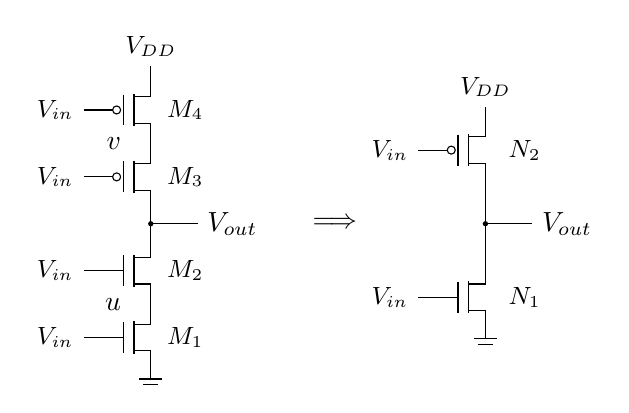
\begin{tikzpicture}[scale=.85]
\mos{0}{0}{V_{in}}{0}\mos{0}{1}{V_{in}}{0}\mos{0}{2.4}{V_{in}}{1}\mos{0}{3.4}{V_{in}}{1}
\draw (.25,1.5)--(.25,1.9);\outputnode{.25}{1.7}{V_{out}}
\rail{.25}{3.9}{V_{DD}}\ground{.25}{-.5}
\node[right,font=\small] at (.35,0){$M_1$};\node[right,font=\small] at (.35,1){$M_2$};
\node[right,font=\small] at (.35,2.4){$M_3$};\node[right,font=\small] at (.35,3.4){$M_4$};
\node[left] at (-.05,.5){$u$};\node[left] at (-.05,2.9){$v$};
\node at (3,1.7){$\Longrightarrow$};
\mos{5}{.6}{V_{in}}{0}\mos{5}{2.8}{V_{in}}{1}
\draw (5.25,1.1)--(5.25,2.3);\outputnode{5.25}{1.7}{V_{out}}
\rail{5.25}{3.3}{V_{DD}}\ground{5.25}{.1}
\node[right,font=\small] at (5.45,.6){$N_1$};\node[right,font=\small] at (5.45,2.8){$N_2$};
\end{tikzpicture}\end{center}

\textbf{(a) $M_1$ and $M_4$ cannot be saturated while their corresponding series paths carry nonzero current.}
For $M_1$ to saturate, $u\ge V_{in}-V_{tn}$. Then
\[
 V_{GS,2}=V_{in}-u\le V_{tn},
\]
so $M_2$ is off (at equality, its ideal overdrive is zero). This contradicts nonzero series current. Thus conducting $M_1$ must be in the linear region. Likewise, saturation of $M_4$ requires
\[
 V_{DD}-v\ge V_{DD}-V_{in}-|V_{tp}| \quad\Longrightarrow\quad v\le V_{in}+|V_{tp}|.
\]
Then $V_{SG,3}=v-V_{in}\le |V_{tp}|$, so $M_3$ is off. Conducting $M_4$ must therefore be linear. $M_2$ and $M_3$, the devices adjacent to the output, can saturate. A cutoff device is not called a conducting saturated device here.

\textbf{(b) Equivalent device sizes.} Two equal, common-gate series devices add their channel lengths in the ideal long-channel, body-effect-free model:
\[
 \boxed{(W/L)_{N_1}=(W/L)_{N_2}=\tfrac12(W/L).}
\]
For example, keep $W$ and use $2L$, or keep $L$ and use $W/2$. In the linear region the two voltage drops sum and yield half the single-device conductance; the same effective $\beta/2$ follows by eliminating the internal node in the square-law saturation equations. This is the ideal static characteristic equivalence intended by the problem. Internal diffusion capacitances and short-channel/body effects prevent a claim of identical physical transient behavior.


\newpage
\section*{2. Multi-threshold CMOS design}
The upper gate in Fig.~2 is XOR, preceded on its $A$ input by an inverter.
Consequently
\[
 U=\bar A,\quad V=\bar B,\qquad
 \boxed{D=U\oplus B=AB+\bar A\bar B},\qquad
 \boxed{E=\overline{BC}}.
\]
With the stated one-unit low-$V_t$ gate delay, the original paths are
$A\to\mathrm{INV}\to\mathrm{XOR}\to D$ (two units),
$B\to\mathrm{XOR}\to D$ (one unit), and
$B,C\to\mathrm{NAND}\to E$ (one unit). The critical delay is two units.
Use low-$V_t$ devices in the $A$ inverter and all devices realizing $D$.
Use high-$V_t$ devices in the four-transistor NAND for $E$, provided its
characterized delay is at most two units. This spends the NAND's one unit
of slack without extending the circuit's maximum delay.

The following complete static CMOS implementation generates both complements
locally. Its XOR core uses the pull-down condition $UB+AV$; the pull-up is
the exact series/parallel dual. All shown thin channels are low-$V_t$;
the four bold NAND channels are high-$V_t$. All pMOS bulks connect to
$\VDD$, and all nMOS bulks to ground. No body-terminal connections are implicit
internal-node ties.
\begin{center}
\resizebox{.98\linewidth}{!}{
\begin{tikzpicture}[font=\small]
 % Inverters for complements.
 \MOS{pa}{1}{4}{A}{p}{.5pt}\MOS{na}{1}{2.4}{A}{n}{.5pt}
 \draw (pat)--(1,4.9) node[above]{$\VDD$};\draw (pab)--(nat);
 \draw (1,3.2)--(2,3.2) node[right]{$U=\bar A$};
 \draw (nab)--(1,1.5) node[below]{$0$};
 \MOS{pb}{4}{4}{B}{p}{.5pt}\MOS{nb}{4}{2.4}{B}{n}{.5pt}
 \draw (pbt)--(4,4.9) node[above]{$\VDD$};\draw (pbb)--(nbt);
 \draw (4,3.2)--(5,3.2) node[right]{$V=\bar B$};
 \draw (nbb)--(4,1.5) node[below]{$0$};
 \node at (2.5,.6) {Complement generators: low-$V_t$};
 % XOR(U,B), equivalent to XNOR(A,B).
 \MOS{p0}{8}{5.5}{U}{p}{.5pt}\MOS{p1}{10.4}{5.5}{B}{p}{.5pt}
 \MOS{p2}{8}{4.2}{A}{p}{.5pt}\MOS{p3}{10.4}{4.2}{V}{p}{.5pt}
 \draw (p0t)--(p1t);\draw (9.2,5.95)--(9.2,6.5) node[above]{$\VDD$};
 \draw (p0b)--(p1b);\draw (p2t)--(p3t);\draw (9.2,5.05)--(9.2,4.65);
 \draw (p2b)--(p3b);\draw (9.2,3.75)--(9.2,3.2)--(11.4,3.2) node[right]{$D$};
 \MOS{n0}{8}{2.4}{U}{n}{.5pt}\MOS{n1}{8}{1.1}{B}{n}{.5pt}
 \MOS{n2}{10.4}{2.4}{A}{n}{.5pt}\MOS{n3}{10.4}{1.1}{V}{n}{.5pt}
 \draw (n0t)--(n2t);\draw (9.2,2.85)--(9.2,3.2);
 \draw (n0b)--(n1t);\draw (n2b)--(n3t);\draw (n1b)--(n3b);
 \draw (9.2,.65)--(9.2,.2) node[below]{$0$};
 \node at (9.2,-.7) {$D$: low-$V_t$ core};
 % NAND E.
 \MOS{ep0}{14}{5}{B}{p}{1.7pt}\MOS{ep1}{16.4}{5}{C}{p}{1.7pt}
 \draw (ep0t)--(ep1t);\draw (15.2,5.45)--(15.2,6) node[above]{$\VDD$};
 \draw (ep0b)--(ep1b);\draw (15.2,4.55)--(15.2,3.6)--(16.8,3.6) node[right]{$E$};
 \MOS{en0}{15.2}{2.8}{B}{n}{1.7pt}\MOS{en1}{15.2}{1.4}{C}{n}{1.7pt}
 \draw (15.2,3.6)--(en0t);\draw (en0b)--(en1t);
 \draw (en1b)--(15.2,.4) node[below]{$0$};
 \node at (15.2,-.5) {$E$: high-$V_t$ NAND};
\end{tikzpicture}}
\end{center}
The added $B$ complement generator is kept low-$V_t$: in this specific static
implementation the $B\to V\to D$ path also takes two gates. Merely selecting
all $B$-controlled XOR devices as high-$V_t$ would be unjustified because
those same series devices can carry a sensitized critical $A$ transition.
The prompt gives no high-$V_t$ delay or leakage parameters, so an unconditional
numerical timing guarantee or leakage reduction cannot be calculated.
If the high-$V_t$ NAND exceeds two units, retain low-$V_t$ devices or resize
and characterize it. The standard CIC018 TT model is not a dual-$V_t$ model.
\texttt{verify\_logic.py} checks all eight $(A,B,C)$ assignments.


\newpage
\section*{3. Multiplexer-based design}
Use $\operatorname{MUX}(s,d_0,d_1)=\bar{s}d_0+sd_1$. Shannon expansion on $x_1$ gives
\[
 f=\bar{x}_1(x_2x_3)+x_1(\bar{x}_2x_3+x_2\bar{x}_3).
\]
The following four 2-to-1 multiplexers implement the function using only true inputs and constants:
\begin{align*}
 n_3&=\operatorname{MUX}(x_3,1,0)=\bar{x}_3,\\
 g_0&=\operatorname{MUX}(x_2,0,x_3)=x_2x_3,\\
 g_1&=\operatorname{MUX}(x_2,x_3,n_3)=x_2\oplus x_3,\\
 f&=\operatorname{MUX}(x_1,g_0,g_1).
\end{align*}
If $\bar{x}_3$ is already available, only the final three MUXes are required.
\begin{center}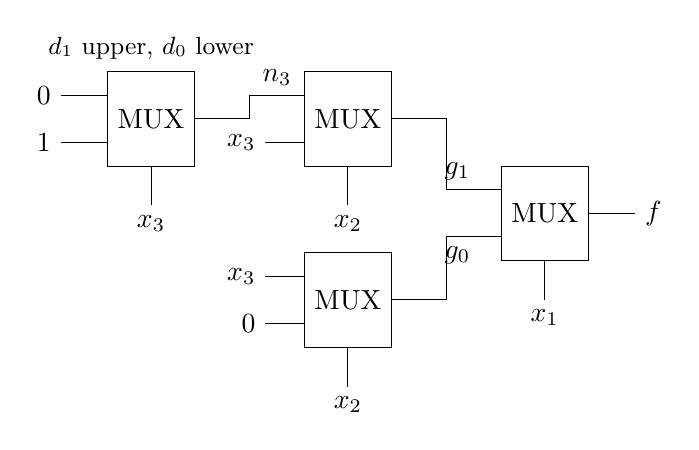
\begin{tikzpicture}[x=1cm,y=1cm]
\draw (0,2) rectangle (1.1,3.2);\node at (.55,2.6){MUX};
\draw (-.6,2.3)--(0,2.3) node[pos=0,left]{$1$};\draw (-.6,2.9)--(0,2.9) node[pos=0,left]{$0$};
\draw (.55,1.5)--(.55,2) node[pos=0,below]{$x_3$};
\draw (2.5,2) rectangle (3.6,3.2);\node at (3.05,2.6){MUX};
\draw (1.1,2.6)--(1.8,2.6)--(1.8,2.9)--(2.5,2.9) node[midway,above]{$n_3$};
\draw (2,2.3)--(2.5,2.3) node[pos=0,left]{$x_3$};\draw (3.05,1.5)--(3.05,2) node[pos=0,below]{$x_2$};
\draw (2.5,-.3) rectangle (3.6,.9);\node at (3.05,.3){MUX};
\draw (2,0)--(2.5,0) node[pos=0,left]{$0$};\draw (2,.6)--(2.5,.6) node[pos=0,left]{$x_3$};
\draw (3.05,-.8)--(3.05,-.3) node[pos=0,below]{$x_2$};
\draw (5, .8) rectangle (6.1,2);\node at (5.55,1.4){MUX};
\draw (3.6,2.6)--(4.3,2.6)--(4.3,1.7)--(5,1.7) node[pos=.2,above]{$g_1$};
\draw (3.6,.3)--(4.3,.3)--(4.3,1.1)--(5,1.1) node[pos=.2,below]{$g_0$};
\draw (5.55,.3)--(5.55,.8) node[pos=0,below]{$x_1$};\draw (6.1,1.4)--(6.7,1.4) node[right]{$f$};
\node[font=\small] at (.55,3.5){$d_1$ upper, $d_0$ lower};
\end{tikzpicture}\end{center}
\begin{center}\begin{tabular}{ccc|c} \toprule $x_1$&$x_2$&$x_3$&$f$\\\midrule
0&0&0&0\\0&0&1&0\\0&1&0&0\\0&1&1&1\\1&0&0&0\\1&0&1&1\\1&1&0&1\\1&1&1&0\\\bottomrule
\end{tabular}\end{center}
The output is 1 exactly when two of the three inputs are 1.

\newpage

\section*{4(a). Static CMOS: $f=\overline{w(x+y)+yz}$}
The pull-down network (PDN) implements $G=w(x+y)+yz$. Its two parallel paths are $n_w$ in series with $(n_x\parallel n_y)$, and $n_y$ in series with $n_z$. The complementary pull-up network (PUN) is
\[
 \bar{G}=[\bar{w}+\bar{x}\bar{y}][\bar{y}+\bar{z}].
\]
Thus use $p_w\parallel(p_x\text{ series }p_y)$, in series with $p_y\parallel p_z$. All gate labels below are true inputs; PMOS devices turn on when their labeled input is 0. Repeated $y$ labels denote distinct transistors. There are 5 PMOS and 5 NMOS devices.
\begin{center}\begin{tikzpicture}[scale=.93]
% PUN top parallel group
\mos{0}{4.1}{w}{1}\mos{2}{4.6}{x}{1}\mos{2}{3.6}{y}{1}
\draw (.25,4.6)--(.25,5.1)--(2.25,5.1);\draw (.25,3.6)--(.25,3.1)--(2.25,3.1);
\mos{0}{2.6}{y}{1}\mos{2}{2.6}{z}{1}
\draw (.25,2.1)--(4.25,2.1);\rail{1.25}{5.1}{V_{DD}}\outputnode{4.25}{2.1}{f}
% PDN left branch W then X/Y
\mos{0}{1.6}{w}{0}\mos{0}{.6}{x}{0}\mos{2}{.6}{y}{0}
\draw (.25,1.1)--(2.25,1.1);\draw (.25,.1)--(.25,-.25)--(4.25,-.25);
\draw (2.25,.1)--(2.25,-.25);
% PDN right branch Y then Z
\mos{4}{1.6}{y}{0}\mos{4}{.6}{z}{0}\draw (4.25,.1)--(4.25,-.25);
\ground{2.25}{-.25}
\node[right,font=\small] at (4.8,4.2){PUN};\node[right,font=\small] at (4.8,.8){PDN};
\end{tikzpicture}\end{center}
Series connections implement AND in a conducting network and parallel connections implement OR. De Morgan's law makes the networks mutually exclusive for every binary input combination: if $G=1$, PDN conducts and PUN does not; if $G=0$, PUN conducts and PDN does not. No input inverter is needed.

\newpage
\section*{4(b). Static CMOS: $f=\bar{x}\bar{y}+\bar{x}\bar{z}+\bar{y}\bar{z}$}
Only true literals are supplied, so form the complement of the desired function for the NMOS gates:
\[
 \bar f=(x+y)(x+z)(y+z)=xy+xz+yz.
\]
Use three series stages, each containing two parallel NMOS devices, for the PDN. The dual PUN has three parallel branches, each containing two series PMOS devices. It contains 6 PMOS and 6 NMOS devices and needs no external complemented inputs.
\begin{center}\begin{tikzpicture}[scale=.93]
\mos{0}{4}{x}{1}\mos{0}{3}{y}{1}
\mos{2}{4}{x}{1}\mos{2}{3}{z}{1}
\mos{4}{4}{y}{1}\mos{4}{3}{z}{1}
\draw (.25,4.5)--(4.25,4.5);\rail{2.25}{4.5}{V_{DD}}
\draw (.25,2.5)--(4.25,2.5);\outputnode{4.25}{2.5}{f}
\draw (.25,2.5)--(.25,2);\draw (2.25,2.5)--(2.25,2);
\mos{0}{1.5}{x}{0}\mos{2}{1.5}{y}{0}
\mos{0}{.5}{x}{0}\mos{2}{.5}{z}{0}
\mos{0}{-.5}{y}{0}\mos{2}{-.5}{z}{0}
\draw (.25,1)--(2.25,1);\draw (.25,0)--(2.25,0);\draw (.25,-1)--(2.25,-1);\ground{1.25}{-1}
\end{tikzpicture}\end{center}
This function is 1 for input Hamming weight 0 or 1 and 0 for weight 2 or 3. The product-of-sums network follows the supplied handwritten solution. An alternative PDN is three parallel two-NMOS stacks ($xy,xz,yz$), with its dual PUN; both implement the same function and use 12 devices.


\section*{Source comparison and reproducibility}
The authentic two-page Fall 2018 HW1 prompt was inspected visually, including
the complete overbar in Q4(a). The supplied three-page handwritten
\texttt{HW1.pdf} was then read. It agrees on the linear-region devices,
half-size static equivalence, Shannon cofactors and complementary CMOS gates.
The present solution adds the nonzero-current qualification, the restrictions
of the ideal long-channel model, the explicit high-$V_t$ NAND delay bound,
and a fourth MUX when the complemented data input is not supplied.
The NAND is the only high-$V_t$ block selected without risking a shared
critical XOR current path. No characterized dual-threshold process models
were supplied, so its timing/leakage condition is theoretical rather than
an asserted CIC018 physical measurement.

The independently authored earlier-year derivations were reused only where
the actual 2018 printed equations and figures match. The reconstructed problem statements and editable circuit diagrams
accompany the independently checked derivations. No missing later
homeworks are inferred from these references.

Run \texttt{python verify\_logic.py}. It verifies 32 original MUX/CMOS cases,
eight dual-$V_t$ block logic cases, and 5,050 square-law stack-equivalence
points. The logic assertions check complementary rail conduction. The
square-law numeric check eliminates the internal stack node and compares
both device currents with an equivalent half-strength device. This is not
a BSIM timing or leakage simulation. CSV truth tables and a JSON summary
are included for reproducibility.
\end{document}
